\chapter{Design and Implementation}

The main goal of this thesis is to extend the current ndnSIM 2.0 implementation in order to allow efficient communication between mobile agents. A first interest packet is broadcast by the consumer on one channel and forwarded by all intermediate nodes in a broadcast manner. Default routes are set by the NFD at the beginning and need to be overridden as soon as more information is obtained. (TODO: need to check how it is on base) Looping interests need to be identified and dropped in order to reduce bandwidth waste. After being forwarded by the intermediate nodes the interest arrives at the producer and a corresponding data packet is created. This packet returns to the consumer and will add routes by updating the FIB entries.

\section{Problem Description}

The current implementation relies only on face id's of the application or net device (\texttt{ndn::NetDevice}) which is sufficient for point to point connections but will not work on wireless communication like in the mobile ad-hoc scenarios investigated in this thesis. Wireless communication is inherently broadcasting and the nodes are responsible to accept the package if it was meant for them and drop it if it was only overheard. There cannot exist a "route" by defining the in-faces of an interest and forwarding it to out-faces obtained from the FIB entries. The same goes for data being forwarded through faces downstream towards a consumer. The topology is not known and changing fast so there needs to be a way to identify specific nodes in a consistent manner.

If one route is found and the FIB entries updated, interests will follow this path to the producer and data will follow the breadcrumbs back to the consumer. That is likely to lead to congestions and incur unnecessary overhead on some of the intermediate nodes while leaving others out of the information flow all together. Having the possibility to chose from different channels and different paths will spread the load onto different intermediate nodes making congestions and retransmissions less likely.


\section{Multipath Approach}

In order to support paths the nodes must know where the packet did come from and for what node is was meant. The faces of the net device cannot be used since they are equal on each node. Every node assigns number id's from 256 to each face. All the nodes will have at least face id 256. Also the application faces will be the same on the consumer and the producer. That can be achieved by using the NDN's net device (\texttt{ndn::NetDevice}) mac addresses that are unique for each simulation. 

\subsection{Changes to the Interest}

In order to have routes and the FIB entries populated, the information about the topology must be communicated to all the surrounding neighbours. The information about previous nodes that have been encountered while forwarding the interest towards a potential content source can be added to the interest. That makes it possible to forward the data downstream towards the requester by following the breadcrumbs left in the PIT entries. These breadcrumbs consist in our implementation of the mac addresses of the net device from the previous node. The interest has three new fields:

\begin{itemize}
\item \emph{std::string m\_interestOriginMacAddress}: This field has the mac address of the previous node.
\item \emph{std::string m\_interestTargetMacAddress}: This field has the mac address of the next node if there is a FIB entry to get the target mac from.
\item \emph{std::string m\_macInterestRoute}: This field shows the the way of the interest so far.
\end{itemize}

The following figure \ref{fig:incomingInterestPipelineWithMac} illustrated the mac address relevant steps in the incoming interest pipeline \texttt{Forwarder::onIncomingInterest}.

\begin{figure}[H]
  \centering
  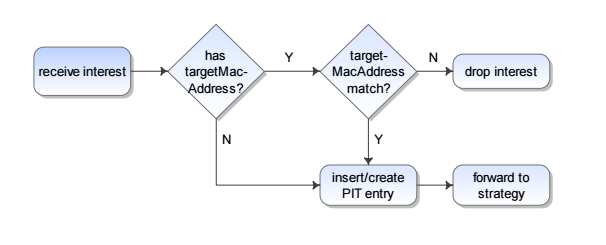
\includegraphics[scale=0.6]{chapter-4/incomingInterestPipelineWithMac}
  \caption{This figure shows how mac addresses are added and checked within the incoming interest pipeline}
  \label{fig:incomingInterestPipelineWithMac}
\end{figure}

At the beginning of the simulation no knowledge about the topology is present. The first interest is broadcast. Since the FIB entries have not yet been populated with information on neighbouring nodes and their mac address, the first interest cannot have a valid targetMacAddress. The missing mac address signals to all receiving nodes that the interest is being flooded through the network and needs to be broadcast further. After information about the topology is present the interest will have a valid mac address of the target it is supposed to reach.

The steps in figure \ref{fig:incomingInterestPipelineWithMac} are the following:

\begin{enumerate}
\item After the node receives the interest, the \emph{Interest::m\_interestTargetMacAddress} is checked for a valid mac address through regular expressions.
\item In the case the interest has no valid target mac address the interest is accepted as broadcast the interest will be inserted into the PIT table with it's origin mac address.
\item If a valid mac address was found, it is checked against the receiving net device's mac address.
\item If the interest's target mac address equals the receiving net device's mac address the interest was meant for this node (in particular to this net device) and will be inserted into the PIT table with it's origin mac address. If the two mac addresses (target mac address and the current device's mac address) do not match the interest was not meant for this node and will be dropped immediately to save resources. No overhearing occurs at any time.
\item The interest will be forwarded to the strategy for further processing.
\end{enumerate}

All interests have valid \emph{std::string m\_interestOriginMacAddress} fields at all time. They are needed to leave the breadcrumbs for the returning data and are inserted into the PIT entries at time of arriving at a new node. If the incoming interest had a valid target mac address, it will become the new (current) mac address of the outgoing interest. If no valid target mac was given to the incoming interest a new current mac address must be chosen from all active net devices. This is done through a static counter and the modulo expresion, making sure, that differenent paths are taken. Adding the new origin mac address happens in \texttt{Forwarder::onOutgoingInterest} or in \texttt{Strategy::afterReceiveInterest}.

\subsection{Changes to the Data}

In order to have routes and the FIB entries populated, the information about the topology must be communicated to all the surrounding neighbours. The data is responsible to populate the FIB entries with this new information and adding mac addresses. Existing FIB entries can be updated or new routes can be added with the help of the \texttt{ns3::ndn::FibHelper} helper class by calling the \texttt(AddRoute) method.

The data is also extended with three new member variables:

\begin{itemize}
\item \emph{std::string m\_dataOriginMacAddress}: This field has the mac address of the previous node.
\item \emph{std::string m\_dataTargetMacAddress}: This field has the mac address of the next node if a mac address was left in the PIT entry.
\item \emph{std::string m\_macDataRoute}: This field shows the the way of the data so far.
\end{itemize}

The following figure \ref{fig:incomingDataPipelineWithMac} illustrated the mac address relevant steps in the incoming data pipeline \texttt{Forwarder::onIncomingData}.

\begin{figure}[H]
  \centering
  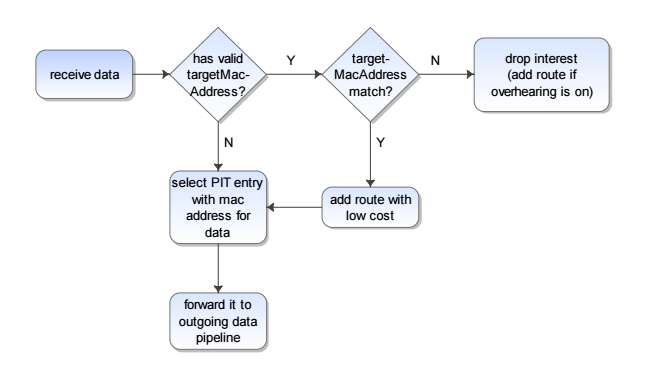
\includegraphics[scale=0.6]{chapter-4/incomingDataPipelineWithMac}
  \caption{This figure shows how mac addresses are added and checked within the incoming data pipeline}
  \label{fig:incomingDataPipelineWithMac}
\end{figure}

The steps are explained as follows:

\begin{enumerate}
\item After the node receives the data, the \emph{Data::m\_dataTargetMacAddress} is checked for a valid mac address through regular expressions.
\item If the target mac address of the data is equal to the current net device's mac address the data was meant for this node. If the mac addresses do not match, the data was overheard.
\item It depends on the implementation if overheard data shall be further processed, cached into CS or just dropped. If it is saved, the route from where it came will be added to the FIB entries for later use.
\item If the data was meant for this node a route is added with low cost, in order to prfioritize the route.
\item From the corresponding PIT entry mac address and face information are retrieved and the added to a copy of the data.
\item The updated copy of the data is then handed off to the outgoing data pipeline.
\end{enumerate}

The outgoing data pipeline is implemented in \texttt{Forwarder::onOutgoingData}. It receives the data with additional parameters. If the target mac address of the data is valid and the data is solicited, the origin mac address field of the data is updated with the correct mac address. If the data was unsolicited a new mac address of the possible net devices is selected in an alternating manner and added to the data. The route is updated and the data is send through it's out-face to the next node.

The data encoding of the interest and data packets had to be extended by the new fields in order to be able to be send over the network and receive by other nodes.

\subsection{Changes to the FIB}

The FIB entries hold information about how to forward the interest upstream. Every FIB entry is uniquely identified by the prefix of the incoming interest. It is found by longest prefix match. The entry aggregates NextHop objects with the corresponding faces and cost information as shown in chapter 3 figure \ref{fig:FIBdataStructure}.
In this thesis it is not done by faces like initially implemented, but by mac addresses. These mac addresses are updated inside existing FIB entries or new FIB entries are created with this additional information. Therefore the new FIB entries have been extended with functions to fetch the new information from the NextHop entries. And the NextHop entries have been extended by a new mac address field.

\begin{figure}[H]
  \centering
  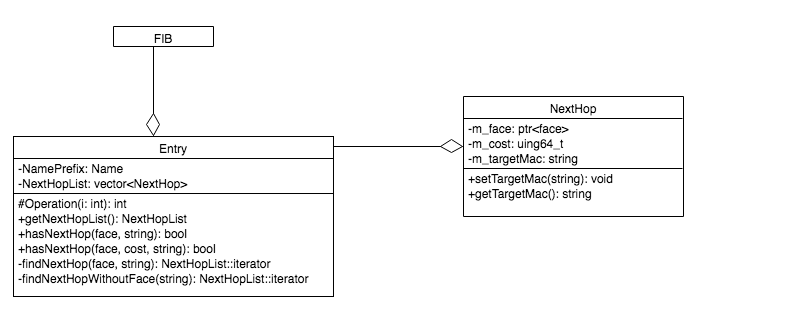
\includegraphics[scale=0.6]{chapter-4/newFIBdataStructure}
  \caption{This figure shows the new FIB data structure}
  \label{fig:newFIBdataStructure}
\end{figure}

Figure \ref{fig:FIBdataStructure} shows only the relevant and new member variables and methods added to the data structure. The FIB entries need new methods that find next hops according to the mac addresses or a combination of mac addresses and faces. A new method returns a NextHopList that is passed by reference and not constant anymore so incrementing on the cost can be done directly on the data structure. The NextHop class has been extended by the target mac field, setters and getters.

\subsection{Changes to the PIT}

The PIT entries hold information about how to forward the data downstream. Every PIT entry is uniquely identified by the prefix of the incoming data. It is found by longest prefix match. The entry aggregates in-record and out-record objects with the corresponding faces lastNonce and lastRenewed information as shown in chapter 3 figure \ref{fig:PITdataStructure}. The faces need to be extended by mac addresses since the data is broadcast and the receiving node needs to identify if it is the intended recipient.

\begin{figure}[H]
  \centering
  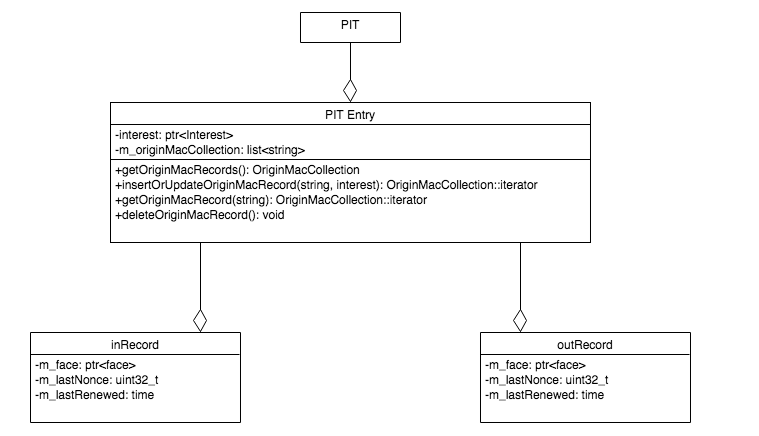
\includegraphics[scale=0.6]{chapter-4/newPITdataStructure}
  \caption{This figure shows the new PIT data structure}
  \label{fig:newPITdataStructure}
\end{figure}

Figure \ref{fig:newPITdataStructure} shows only the relevant and new member variables and methods added to the data structure. A new list member variable \texttt{m\_originMacCollection} has been added to the PIT entry. Every interest forwarded correctly leaves it's origin mac address in this list. When requested data comes it checks the origin mac collection in the PIT entry and attaches it to the data's field. Methods, setters and getters encapsulate the member variable within it's class.

\section{Retransmissions}

(TODO: every retransmission should be broadcast in order to tackle the ad-hoc component)

\section{Mobility}

explain trace-files....
